\documentclass{standalone}
\usepackage[usenames,dvipsnames]{xcolor}
\usepackage{tikz}
\usetikzlibrary{calc,fadings,decorations.pathreplacing}
\usepackage{amsmath}
\definecolor{Set1-5-1}{RGB}{228,26,28} %Red
\definecolor{Set1-5-2}{RGB}{55,126,184} %Blue
\begin{document}
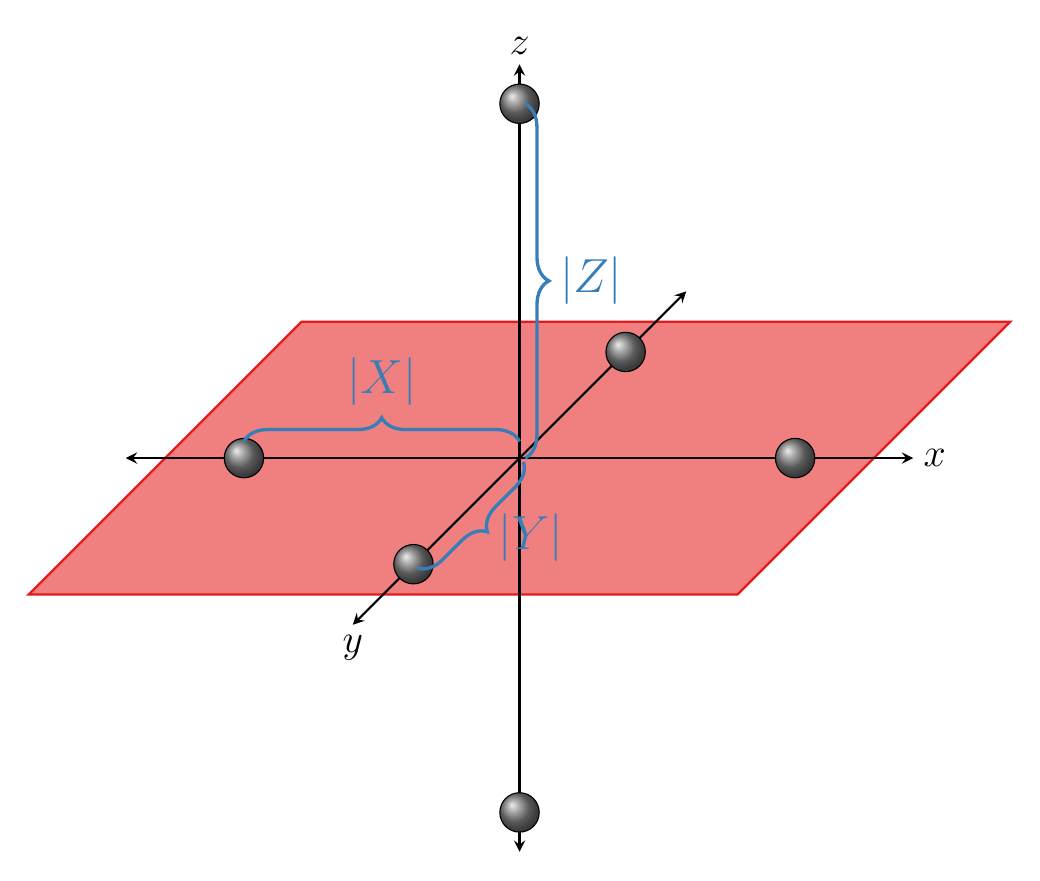
\begin{tikzpicture}
%\definecolor{comp}{RGB}{62,152,204}
%Oxygen plane
\filldraw[thick,Set1-5-1,fill=Set1-5-1!80,fill opacity=0.7] (0.5,5,-4.5) -- (0.5,5,4.5) -- (9.5,5,4.5) -- (9.5,5,-4.5) -- cycle;
%Axes
\draw[stealth-stealth,thick] (0,5) -- (10,5) node[right] {\Large $x$}; %x
\draw[stealth-stealth,thick] (5, 0) -- (5,10) node[above] {\Large $z$}; %y
\draw[stealth-stealth,thick] (5,5,-5.5) -- (5,5,5.5) node[below] {\Large $y$}; %z
%Aluminium
\shadedraw [ball color = gray] (5,0.5,0) circle (0.25);
\shadedraw [ball color = gray] (5,9.5,0) circle (0.25);
\shadedraw [ball color = gray] (1.5,5,0) circle (0.25); %0.625
\shadedraw [ball color = gray] (8.5,5,0) circle (0.25); %9.375
\shadedraw [ball color = gray] (5,5,-3.5) circle (0.25);
\shadedraw [ball color = gray] (5,5,3.5) circle (0.25);

%labels
\draw[very thick,Set1-5-2,decorate,decoration={brace,raise=6pt,amplitude=2ex}] (1.5,5) -- (5,5)
       node[midway,above=3.5ex] {\LARGE $\lvert X\rvert$};
\draw[very thick,Set1-5-2,decorate,decoration={brace,raise=2pt,amplitude=2ex}] (5,5,0) -- (5,5,3.5)
       node[near end,right=4ex] {\LARGE $\lvert Y\rvert$};
\draw[very thick,Set1-5-2,decorate,decoration={brace,raise=2pt,amplitude=2ex}] (5,9.5) -- (5,5)
       node[midway,right=2.5ex] {\LARGE $\lvert Z\rvert$};
\end{tikzpicture}
\end{document} 